\section*{Общая характеристика работы}

\newcommand{\actuality}{\underline{\textbf{\actualityTXT}}}
\newcommand{\progress}{\underline{\textbf{\progressTXT}}}
\newcommand{\aim}{\underline{{\textbf\aimTXT}}}
\newcommand{\tasks}{\underline{\textbf{\tasksTXT}}}
\newcommand{\novelty}{\underline{\textbf{\noveltyTXT}}}
\newcommand{\influence}{\underline{\textbf{\influenceTXT}}}
\newcommand{\methods}{\underline{\textbf{\methodsTXT}}}
\newcommand{\defpositions}{\underline{\textbf{\defpositionsTXT}}}
\newcommand{\reliability}{\underline{\textbf{\reliabilityTXT}}}
\newcommand{\probation}{\underline{\textbf{\probationTXT}}}
\newcommand{\contribution}{\underline{\textbf{\contributionTXT}}}
\newcommand{\publications}{\underline{\textbf{\publicationsTXT}}}

Жидкие кристаллы (ЖК) представляют собой вещества, сочетающие в себе свойства жидкостей и твёрдых тел.
С одной стороны, они способны течь, как вязкие жидкости; с другой стороны, им присуща анизотропия, свойственная кристаллам.
Наиболее исследованными среди них являются нематики, или нематические жидкие кристаллы (НЖК), и холестерики, или холестерические жидкие кристаллы (ХЖК).
Чаще всего молекулы этих веществ имеют вытянутую (стержневидную, конусовидную, каплевидную) форму.
Направление вдоль вытянутой оси молекулы можно обозначить единичным вектором $\textbf{a}$.
Кроме того, существует ещё один класс веществ, у которых наблюдается нематическая или холестерическая упорядоченность.
Это вещества, образованные дискообразными молекулами; в этом случае вектор $\textbf{a}$ направлен также вдоль оси симметрии молекулы.
Усреднение векторов $\textbf{a}$ по физически бесконечно малому объёму после нормировки даёт единичный вектор $\textbf{n}$, называемый директором.
Директор $\textbf{n}$ является важной переменной, позволяющей описывать искажения структуры жидкого кристалла в рамках механики сплошной среды.
Подчеркнём, что в среде выделенной является ось, а не направление, поэтому направления $\textbf{n}$ и $-\textbf{n}$ физически эквивалентны.
При температурах выше некоторой критической ЖК находятся в изотропной фазе, в которой нет выделенного направления, а при температуре ниже критической -- в упорядоченной фазе, в которой директор показывает направление преимущественной ориентации молекул в окрестности данной точки.
Главное отличие НЖК от ХЖК в том, что при температуре ниже критической и в отсутствие внешних воздействий молекулы НЖК выстраиваются вдоль некоторой оси, в то время как молекулы ХЖК образуют так называемую планарную геликоидальную структуру -- периодическую спиральную структуру вдоль некоторого направления в пространстве.
При этом директор $\textbf{n}$ равномерно поворачивается при перемещении вдоль этого направления, оставаясь ему перпендикулярным.
\begin{figure}
	\begin{minipage}{0.49\textwidth}
		\centering
		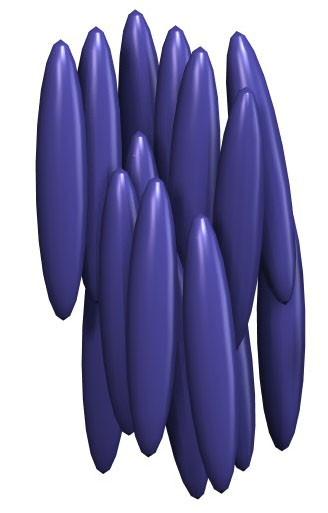
\includegraphics[height=7cm, width=\textwidth]{Nematic_example}
		{А}
	\end{minipage}
	\hfill
	\begin{minipage}{0.49\textwidth}
		\centering
		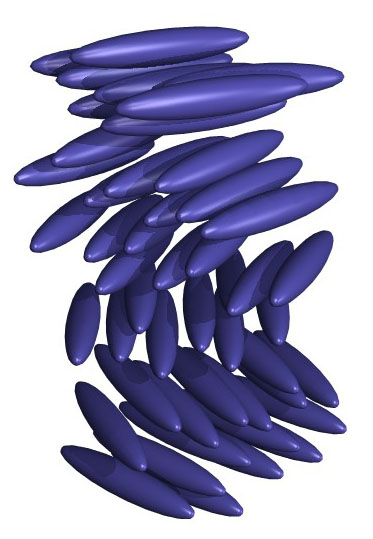
\includegraphics[height=7cm, width=\textwidth]{Cholesteric_example}
		{Б}
	\end{minipage}
	\vspace{0.5cm}
	\caption{Схематическое изображение НЖК (А) и ХЖК (Б)}
\end{figure}

Важной особенностью ЖК является способность к переориентации во внешнем поле, как в магнитном, так и в электрическом.
Это явление, открытое в 1927 году, называется эффектом Фредерикса~\autocite{Fred1927,Fred1933}.
%Примером устройства, в основе работы которого лежит эффект Фредерикса, может служить \todo{TND (twisted nematic device)}
Именно это свойство позволяет использовать ЖК для создания различных электрооптических устройств: систем вывода информации (дисплеев), переключаемых дифракционных решёток, очков и окон с изменяемой светопропускной способностью, беззеркальных лазеров и т.д.~\cite{Blinov1994, McManamon1996, Taheri2000, F.2001, Schmidtke2003, Senyuk2005, Jiang2019}.

Несмотря на то, что эффект Фредерикса изучался в течение долгого времени и для ряда случаев описан как теоретически, так и экспериментально для различных фаз: нематической, холестерической и т.д.~\cite{pikin, deGennesbook1995, stewartBook}, в последнее десятилетие интерес к его изучению возрос~\cite{Brown2003, Brown2007, Makarov2010, Garbovskiy2017, dosSantos2019, Begum2020}.
Большинство исследований идут в сторону усложнения систем и условий, в которых они находятся: рассматриваются различные типы ЖК, геометрии ячеек и граничные условия.
Это в первую очередь связано с возможностью создания систем, обладающих заданными свойствами для потенциальных технических приложений.
При этом наибольший интерес представляют напряжения, индуцирующие переход, а также трансформация равновесной структуры при напряжении выше порогового, так как именно от пространственного распределения директора зависят оптические свойства ячейки.
Важно отметить, что теоретические описания перехода Фредерикса значительно отличаются для магнитного и электрического полей, так как электрическое поле оказывается неоднородным внутри ячейки ЖК~\autocite{Deuling,NonHomoElectricField1972,CTBerr,Arakelyan1984,Napoli2006}.
Ранее переход Фредерикса в нематиках рассматривался как фазовый переход второго рода~\autocite{Guyon1975}, то есть непрерывный фазовый переход.
Однако оказалось, что в киральных нематиках (холестериках) этот переход может быть как непрерывным, так и разрывный, в зависимости от значений материальных констант~\autocite{VAR2013}.

Ещё одно важное свойство ЖК заключается в появлении дополнительной поляризации в результате искажения поля директора.
Такую поляризацию называют \textit{флексоэлектрической}.
%Поляризацию, появляющуюся в ЖК в результате искажения поля директора, называют \textit{флексоэлектрической}.
Флексоэлектрический эффект бывает как прямым, так и обратным. \todo{Так, прямой эффект представляет собой появление добавочной поляризации при искажении структуры образца. Обратному же флексоэлектрическому эффекту соответствует появление искажений в структуре образца под действием электрического поля.}
\textcolor{blue}{(Это надо пояснить, так как без флексоэлектричества, только за счёт диэлектрической поляризации структура в поле меняется, и получаем переход Фредерикса. А вообще, надо ли говорить об обратном эффекте?)}
Первым теоретически описал это явление Майер в 1969 году~\cite{Meyer1969}.
Он дал объяснение~\textit{дипольному} механизму появления флексоэлектрической поляризации для молекул клино- или банановидной формы, обладающих собственным дипольным моментом (см. Рис.~\ref{pic-Meyer}). 

\begin{figure}[ht]
	\centering
	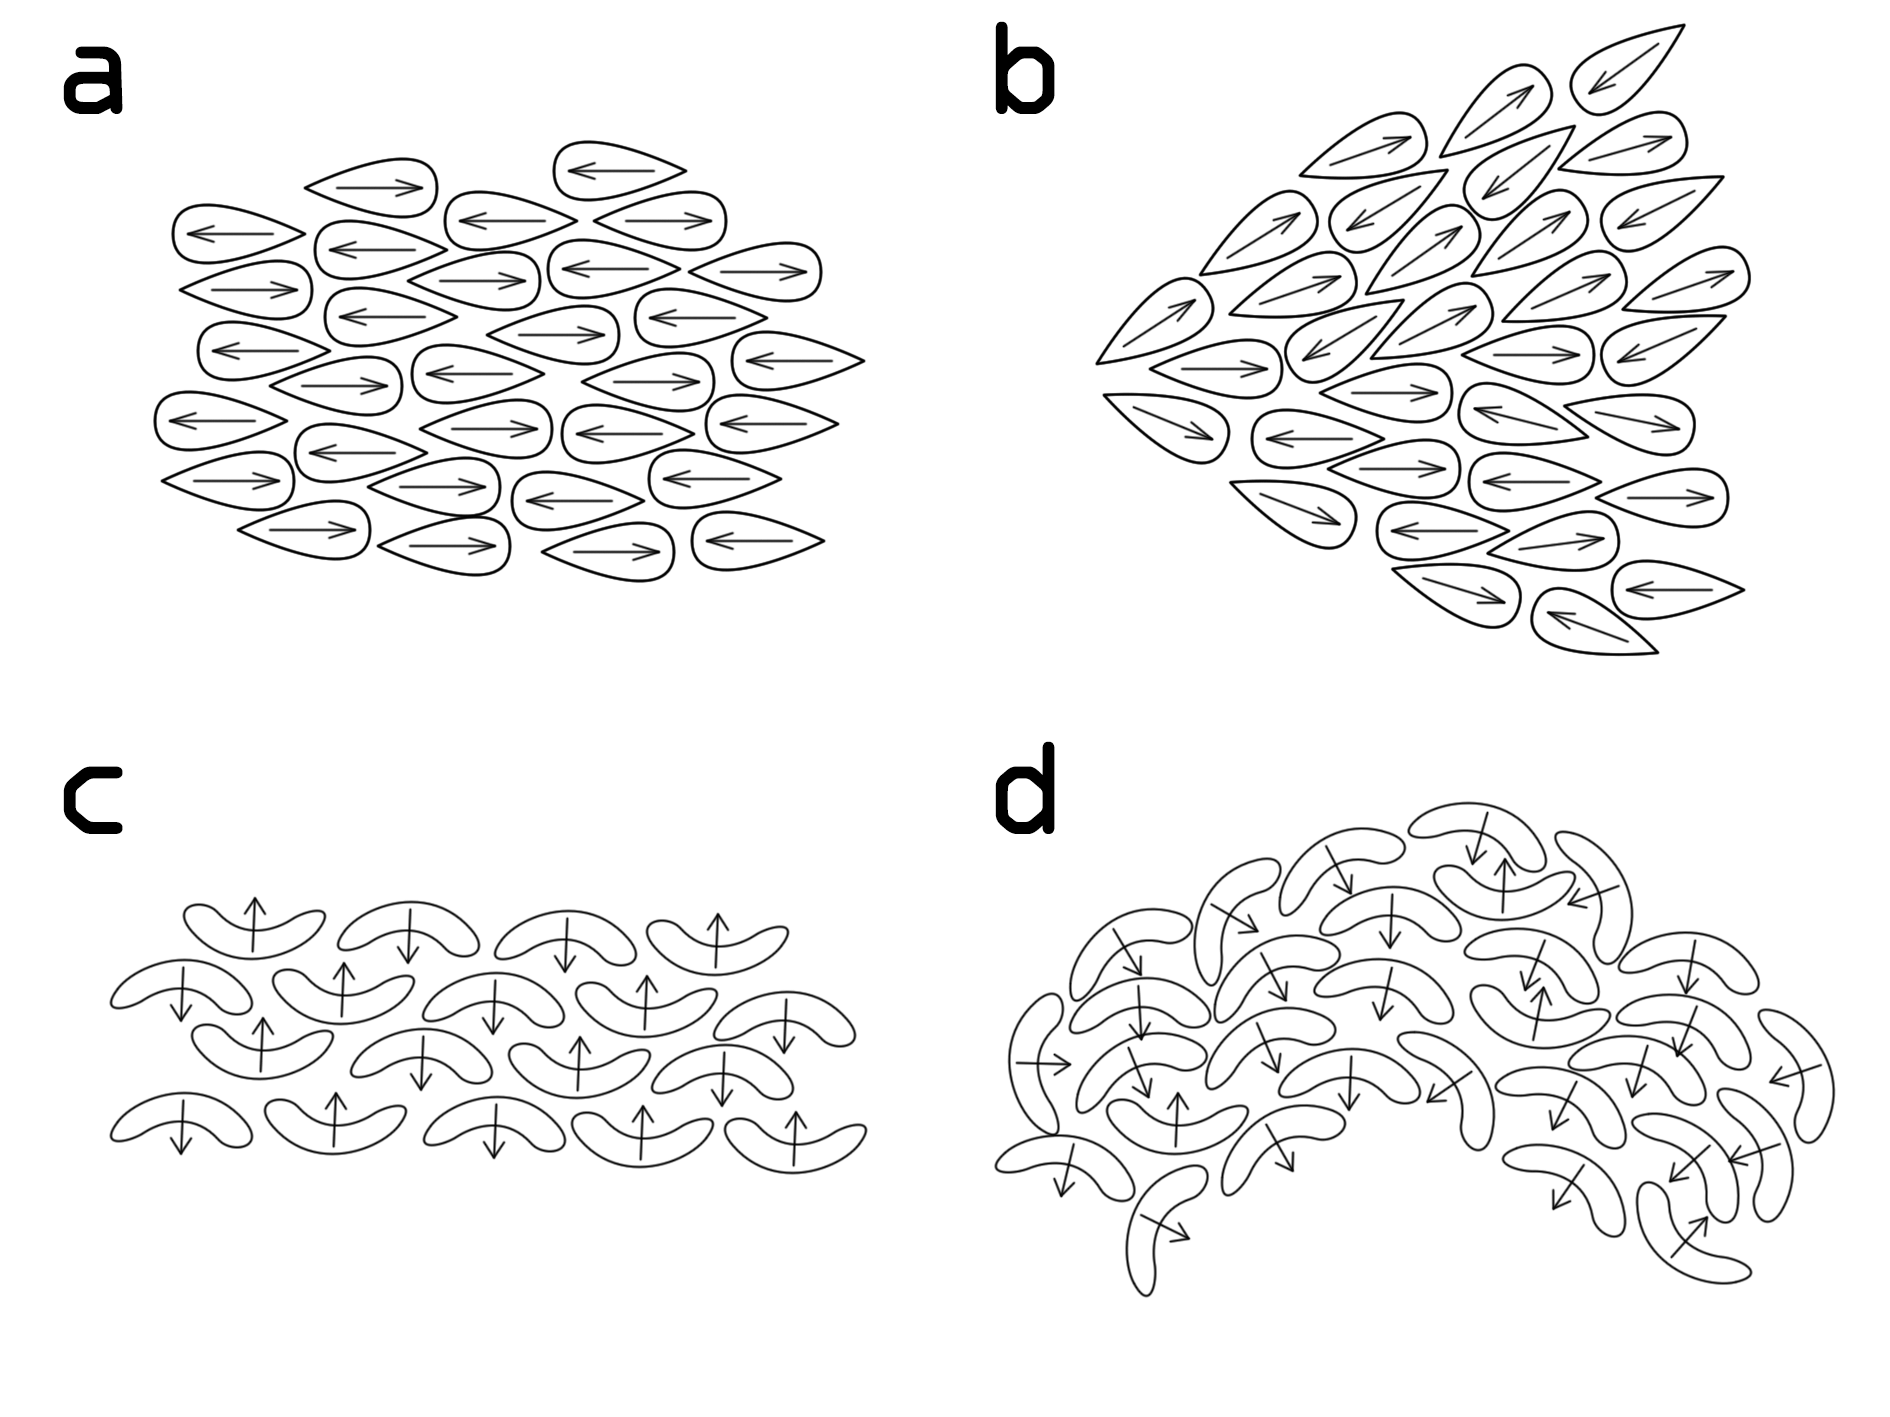
\includegraphics[width=14cm]{Molecules}
	\caption{Появление флексоэлектрической поляризации у молекул специальной формы. Неискажённые состояния для молекул соответственно клиновидной (a) и банановидной (c) формы. Поперечный изгиб, флексоэлектрическая поляризация направлена вправо (b). Продольный изгиб, флексоэлектрическая поляризация направлена вниз (d).}
	\label{pic-Meyer}
\end{figure}

Однако, как показал Прост в 1977 году, этот механизм не является единственным~\cite{Prost77}.
Он объяснил второй известный ныне механизм флексоэлектричества -- квадрупольный.
На рис.~\ref{Prost_explanation}a изображена неискажённая структура из молекул, не обладающих собственным дипольным моментом, но обладающих квадрупольным моментом, причём поляризация в каждом слое равна нулю.
На рис.~\ref{Prost_explanation}b изображена группа таких же молекул, которые подвержены деформации поперечного изгиба.
Видно, что в верхней части области 2 положительный заряд увеличен за счёт квадруполя из области 1.
В то же время, положительный заряд внизу области 2 уменьшился за счёт того, что квадруполи частично перешли в область 3.
Таким образом, данная структура начинает обладать собственным дипольным моментом, направленным вверх, и к ней можно применить всё то, что было сказано про полярные молекулы.
\begin{figure}[ht]
	\centering
	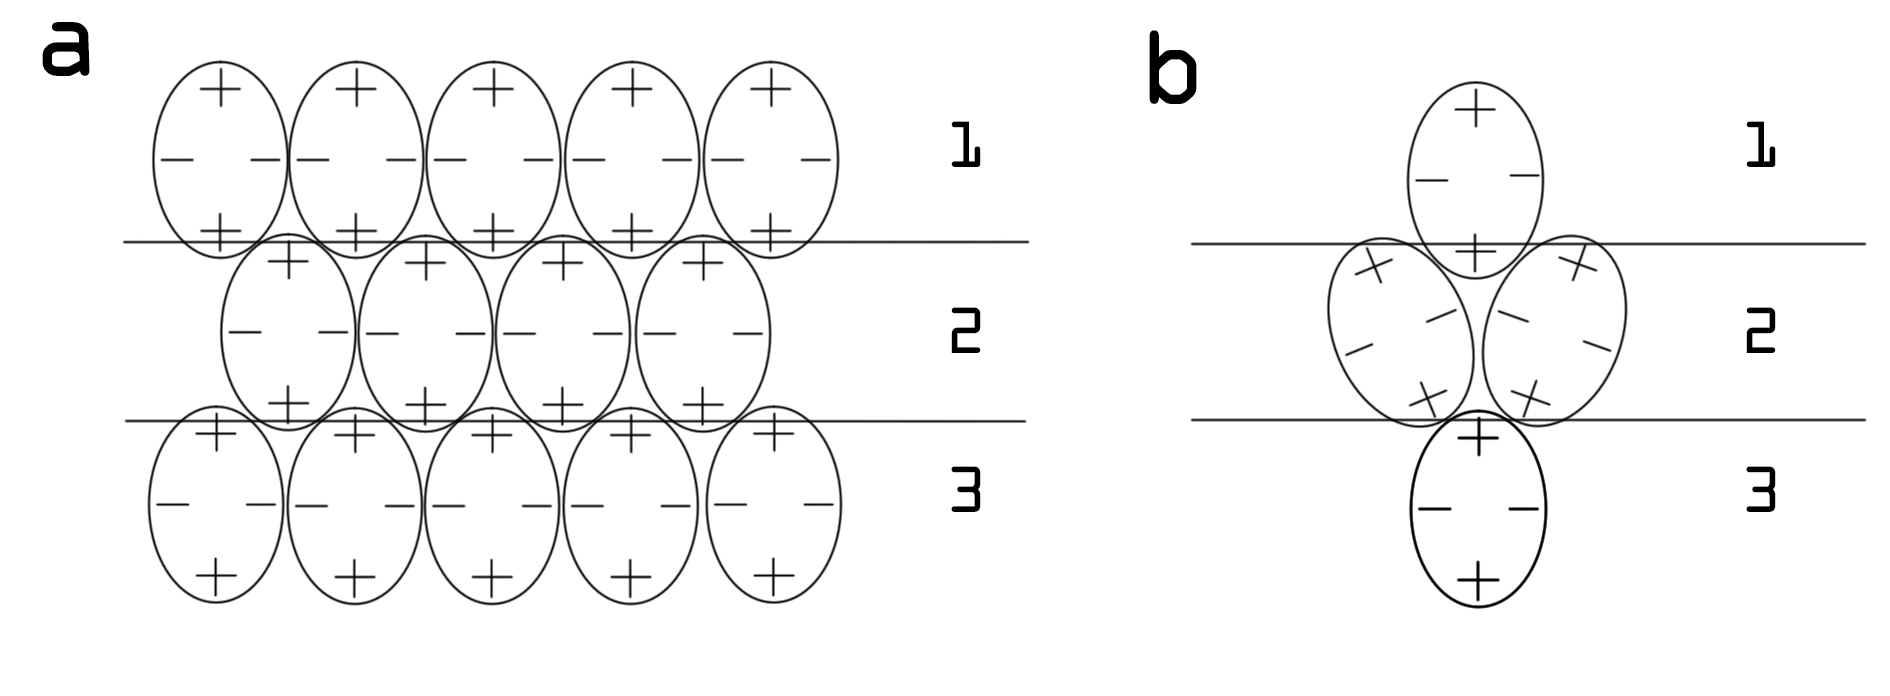
\includegraphics[width=17cm]{Prost_explanation}
	\caption{Симметричные молекулы -- поперечный изгиб}
	\label{Prost_explanation}
\end{figure}

\textcolor{blue}{(До слов о данной работе надо поместить обзор того что делалосьпри изучении Фред.  С учётом и без учёта флекса, неоднородности поля, сцепления с границами, разных геометрий ячеек, наличия ионных примесей, временных характеристик, и всего, что изучают в нематиках и ХЖК. После этого прояснится место этой работы)}

Данная работа посвящена изучению влияния внешнего электрического поля на ориентационную структуру ХЖК с учётом флексоэлектрического эффекта.
\textcolor{blue}{В отсутствие внешних воздействий равновесная структура ХЖК представляет собой планарную геликоидальную структуру: в любой плоскости, перпендикулярной некоторой оси, директор распределён равномерно, а вдоль этой оси распределение имеет вид пространственной спирали, в котором директор равномерно вращается вокруг оси. ЭТО ПОВТОР. Надо из обеих частей взять лучшее, а остальное убрать.}
\todo{РИСУНКИ.}
Если ХЖК находится в контакте с ориентирующей поверхностью, то направление оси, определяющей пространственное вращение директора, может быть зафиксировано.
В данной работе изучается ячейка, представляющая собой две проводящие плоскопараллельные пластины, пространство между которыми заполнено ХЖК, и ось спирали перпендикулярна ограничивающим плоскостям.
Особенность данной работы в том, что производится учёт вклада \textit{флексоэлектрической поляризации} в свободную энергию ХЖК. \textcolor{blue}{(Здесь это выглядит как-то неуместно)}

\todo{АО: не знаю, куда поставить, пусть пока тут побудет. В поиске равновесной структуры ХЖК помогает одно из её общих свойств -- она должна минимизировать соответствующий термодинамический потенциал. Так как объём, температура, а также количество частиц в рассматриваемой системе постоянно, в качестве термодинамического потенциала выбирается свободная энергия.}

В данной работе исследуется влияние флексоэлектрической поляризации на напряжение, индуцирующее переход Фредерикса в ХЖК при различных параметрах системы, таких как сумма флексоэлектрических коэффициентов, жёсткие и мягкие, симметричные и несимметричные граничные условия и др. В первом разделе рассмотрено выражение для свободной энергии ХЖК, отдельно рассмотрен вклад флексоэлектрической поляризации. Во втором разделе получены уравнения Эйлера-Лагранжа на равновесную конфигурацию ХЖК, исключён из описания азимутальный угол. При помощи численной минимизации функционала свободной энергии найдены равновесные конфигурации при различных условиях. В третьем разделе рассматривается устойчивость основного состояния ХЖК (планарной геликоидальной структуры). В четвёртом разделе при помощи теории Ландау и разложения энергии по низшей гармонике оценено критическое поле перехода Фредерикса и проанализирован характер перехода. В пятом разделе подведены итоги исследования.

\if 0
\todo{РАЗДЕЛИТЕЛЬ}
Эффект молекулярной переориентации в ячейках жидких кристаллов (ЖК), вызванной внешним полем, широко исследуется, во многом благодаря многообразию приложений.
Это явление, известное как переход (эффект) Фредерикса \textcolor{blue}{был открыт в конце 1920-х годов.(ссылки)}
Среди устройств, в основе работы которых лежит эффект Фредерикса, можно выделить, например, ЖК-дисплеи, переключаемые дифракционные решётки, беззеркальные лазеры и другие~\autocite{YangWu2014}. 
Переход Фредерикса изучался для различных полей: статического электрического и магнитного полей, осциллирующего электрического поля, лазерного излучения, а также для ЖК в различных фазах: нематической, холестерической, смектической и т.~д.~\autocite{Blinov1994,deGennesbook1995,stewartBook}

Простейшим способом учёта взаимодействия с границами является случай жёстких граничных условий.
Слабое зацепление обычно описывается потенциалом Рапини-Папулара~\autocite{Rapini69}.
Важно отметить, что теоретические описания перехода Фредерикса значительно отличаются для магнитного и электрического полей, так как электрическое поле оказывается неоднородным внутри ячейки ЖК~\autocite{Deuling,NonHomoElectricField1972,CTBerr,Arakelyan1984,Napoli2006}.
Ранее переход Фредерикса в нематиках рассматривался как фазовый переход второго рода~\autocite{Guyon1975}, то есть непрерывный фазовый переход.
Однако оказалось, что в киральных нематиках (холестериках) этот переход может быть как непрерывным, так и \todo{разрывный}, в зависимости от материальных констант~\autocite{VAR2013}.

В последнее время наблюдается растёт интерес к изучению влияния флексоэлектричества~\autocite{buka2012flexoelectricity} на пороговые эффекты в ЖК, например, на переключение бистабильных ЖК-устройств~\autocite{Davidson2002,  Parry-Jones2009, Cummings2013}.
Благодарю флексоэлектричеству возникает дополнительное искажение электрического поля, таким образом, оно тоже влияет на переход Фредерикса.
Такой переход в нематических ЖК (НЖК) изучался в работах~\autocite{Brown2003,Brown2007,Mema2017}.
Анализ при этом ограничивался жёсткими граничными условиями, а также приближением низшей гармоники для объёмного распределения директора и электрического поля.

\todo{ДАЛЬШЕ -- ЧТО СДЕЛАНО В РАБОТЕ PRE2018}
Данная работа посвящена теоретическому изучению перехода Фредерикса в случае статического электрического поля в плоскопараллельной ячейке холекстерического ЖК (ХЖК) с учётом флексоэлектрического эффекта, конечной энергии зацепления, а также неоднородности электрического поля внутри ячейки.
При этом задача состоит в нахождении следующих параметров: пороговые напряжения, равновесная конфигурация директора при напряжении выше напряжения перехода \todo{[просто равновесной конфигурации директора?]}, а также род перехода.
Отдельный акцент сделан на устойчивости равновесных структур, а также на построении фазовых диаграмм.

Работа построена следующим образом. В \todo{Секции $N$} выводится выражение для свободной энергии плоскопараллельной ячейки ЖК\todo{, подключённой к источнику}\todo{[, в виде суммы поверхностных и объёмных вкладов]}.
При этом учитывается неоднородность электрического поля внутри ячейки, вызванная диэлектрической анизотропией ЖК и флексоэлектричеством.
Поверхностная свободная энергия описывается потенциалом Рапини-Папулара.
В \todo{Секции $N+1$} находится равновесное распределение директора для широкого спектра материальных констант.
Также при помощи численного вариационного анализа построены фазовые диаграммы, включая зоны стабильности и метастабильности.
В \todo{Секции $N+2$} аналитически изучается устойчивость планарной геликоидальной структуры.
В \todo{Секции $N+3$} исследуется род перехода Фредерикса с использованием двухпараметрической модели Ландау.
В \todo{Секции $N+4$} содержится подведение итогов и обсуждение результатов.
% Счётчик \texttt{citeexternal} используется для подсчёта процитированных публикаций.
\fi
 % Характеристика работы по структуре во введении и в автореферате не отличается (ГОСТ Р 7.0.11, пункты 5.3.1 и 9.2.1), потому её загружаем из одного и того же внешнего файла, предварительно задав форму выделения некоторым параметрам

%Диссертационная работа была выполнена при поддержке грантов \dots

%\underline{\textbf{Объем и структура работы.}} Диссертация состоит из~введения,
%четырех глав, заключения и~приложения. Полный объем диссертации
%\textbf{ХХХ}~страниц текста с~\textbf{ХХ}~рисунками и~5~таблицами. Список
%литературы содержит \textbf{ХХX}~наименование.

\section*{Содержание работы}
Во \underline{\textbf{введении}} обосновывается актуальность
исследований, проводимых в~рамках данной диссертационной работы,
приводится обзор научной литературы по изучаемой проблеме,
формулируется цель, ставятся задачи работы, излагается научная новизна
и практическая значимость представляемой работы. В~последующих главах
сначала описывается общий принцип, позволяющий \dots, а~потом идёт
апробация на частных примерах: \dots  и~\dots.


\underline{\textbf{Первая глава}} посвящена \dots

 картинку можно добавить так:
\begin{figure}[ht]
  \centerfloat{
    \includegraphics[scale=0.27]{latex}
  }
  \caption{Подпись к картинке.}\label{fig:latex}
\end{figure}

Формулы в строку без номера добавляются так:
\[
  \lambda_{T_s} = K_x\frac{d{x}}{d{T_s}}, \qquad
  \lambda_{q_s} = K_x\frac{d{x}}{d{q_s}},
\]

\underline{\textbf{Вторая глава}} посвящена исследованию

\underline{\textbf{Третья глава}} посвящена исследованию

Можно сослаться на свои работы в автореферате. Для этого в файле
\verb!Synopsis/setup.tex! необходимо присвоить положительное значение
счётчику \verb!\setcounter{usefootcite}{1}!. В таком случае ссылки на
работы других авторов будут подстрочными.
Изложенные в третьей главе результаты опубликованы в~\cite{vakbib1, vakbib2}.
Использование подстрочных ссылок внутри таблиц может вызывать проблемы.

В \underline{\textbf{четвертой главе}} приведено описание

В \underline{\textbf{заключении}} приведены основные результаты работы, которые заключаются в следующем:
\input{common/concl}

При использовании пакета \verb!biblatex! список публикаций автора по теме
диссертации формируется в разделе <<\publications>>\ файла
\verb!common/characteristic.tex!  при помощи команды \verb!\nocite!

\ifdefmacro{\microtypesetup}{\microtypesetup{protrusion=false}}{} % не рекомендуется применять пакет микротипографики к автоматически генерируемому списку литературы
\urlstyle{rm}                               % ссылки URL обычным шрифтом
\ifnumequal{\value{bibliosel}}{0}{% Встроенная реализация с загрузкой файла через движок bibtex8
  \renewcommand{\bibname}{\large \bibtitleauthor}
  \nocite{*}
  \insertbiblioauthor           % Подключаем Bib-базы
  %\insertbiblioexternal   % !!! bibtex не умеет работать с несколькими библиографиями !!!
}{% Реализация пакетом biblatex через движок biber
  % Цитирования.
  %  * Порядок перечисления определяет порядок в библиографии (только внутри подраздела, если `\insertbiblioauthorgrouped`).
  %  * Если не соблюдать порядок "как для \printbibliography", нумерация в `\insertbiblioauthor` будет кривой.
  %  * Если цитировать каждый источник отдельной командой --- найти некоторые ошибки будет проще.
  %
  %% authorvak
  \nocite{vakbib1}%
  \nocite{vakbib2}%
  %
  %% authorwos
  \nocite{wosbib1}%
  %
  %% authorscopus
  \nocite{scbib1}%
  %
  %% authorconf
  \nocite{confbib1}%
  \nocite{confbib2}%
  %
  %% authorother
  \nocite{bib1}%
  \nocite{bib2}%

  \ifnumgreater{\value{usefootcite}}{0}{
    \begin{refcontext}[labelprefix={}]
      \ifnum \value{bibgrouped}>0
        \insertbiblioauthorgrouped    % Вывод всех работ автора, сгруппированных по источникам
      \else
        \insertbiblioauthor      % Вывод всех работ автора
      \fi
    \end{refcontext}
  }{
  \ifnum \value{citeexternal}>0
    \begin{refcontext}[labelprefix=A]
      \ifnum \value{bibgrouped}>0
        \insertbiblioauthorgrouped    % Вывод всех работ автора, сгруппированных по источникам
      \else
        \insertbiblioauthor      % Вывод всех работ автора
      \fi
    \end{refcontext}
  \else
    \ifnum \value{bibgrouped}>0
      \insertbiblioauthorgrouped    % Вывод всех работ автора, сгруппированных по источникам
    \else
      \insertbiblioauthor      % Вывод всех работ автора
    \fi
  \fi
  %  \insertbiblioauthorimportant  % Вывод наиболее значимых работ автора (определяется в файле characteristic во второй section)
  \begin{refcontext}[labelprefix={}]    \insertbiblioexternal            % Вывод списка литературы, на которую ссылались в тексте автореферата
  \end{refcontext}
  }
}
\ifdefmacro{\microtypesetup}{\microtypesetup{protrusion=true}}{}
\urlstyle{tt}                               % возвращаем установки шрифта ссылок URL
